\chapter{Estado del arte}\label{sec:estadodelarte}

\paragraph{}En este capítulo vamos a tratar sobre el estado actual de las tecnologías
más relevantes para llevar a cabo entornos de desarrollo replicables, flexibles y universales.
Explicaremos que aspectos son los más interesantes en cada caso y como podrían aplicarse.

\section{Yocto Project.}\label{sec:yocto}

\paragraph{} \emph{Yocto Project} es un proyecto colaborativo y de código abierto
de la \emph{Linux Foundation} cuyo objetivo principal es la producir herramientas y
procesos que permitan crear distribuciones embebidas de sistemas operativos basados
en el Kernel de Linux. Su código está pensado para que las herramientas y las distribuciones
generadas sean agnósticas respecto de la arquitectura del microprocesador así como del
resto del hardware.
\cite{yoctoprojectpage}

\begin{figure}[h]
	\centering
	
\includegraphics[width=0.35\linewidth]{imgs/yocto-logo}
	\caption[Logo Yocto Project]{Yocto Project. Un proyecto de la Linux Fundation}
	\label{fig:yocto_logo}
\end{figure}

\paragraph{} Yocto es, por tanto, una excelente herramienta para asegurar la repetibilidad
de los sistemas, así como para asegurar la seguridad de los mismos, al tiempo de ser capaz
de ser flexible y parametrizable. Decimos que es bueno para asegurar la repetibilidad
ya que la empresa toma posesión del sistema operativo entero y deja de depender de
distribuciones de terceros que puedan introducir cambios sin previo aviso. Asegura la
seguridad ya que tiene un gran soporte que de la comunidad \emph{\gls{open source}} cercana
al desarrollo del propio kernel de Linux, proporcionando rápidamente los últimos parches
de seguridad que se publican. Es flexible ya que permite adaptar cualquier los cambio
introducido en el hardware, manteniendo antiguas versiones o incluso desarrollar más de
un hardware al mismo tiempo. Esto es un gran ventaja en los tiempo en los que los equipos
de software deben empezar su código sin tener un sistema hardware final, donde incluso
se desarrolle parte del hardware es dispositivos basado en \emph{\gls{FPGAs}}.

\paragraph{} Este proyecto que fue fundado en 2010 con el apoyo de grandes multinacionales
y organizaciones. Destaca la estrecha colaboracioón con \emph{OpenEmbedded}, tomando de
ellos la mayor parte del \emph{OpenEmbedded Project} y su motor de generación (\emph{build
engine}), bitbake.

\paragraph{} Como parte del proyecto, con cada versión de Yocto, se presenta una versión
de Poky. Poky, es una distribuición de referencia, a partir de la cual, puedes basarte
para la construción de tu distribución propia.

\begin{figure}[h]
	\centering
	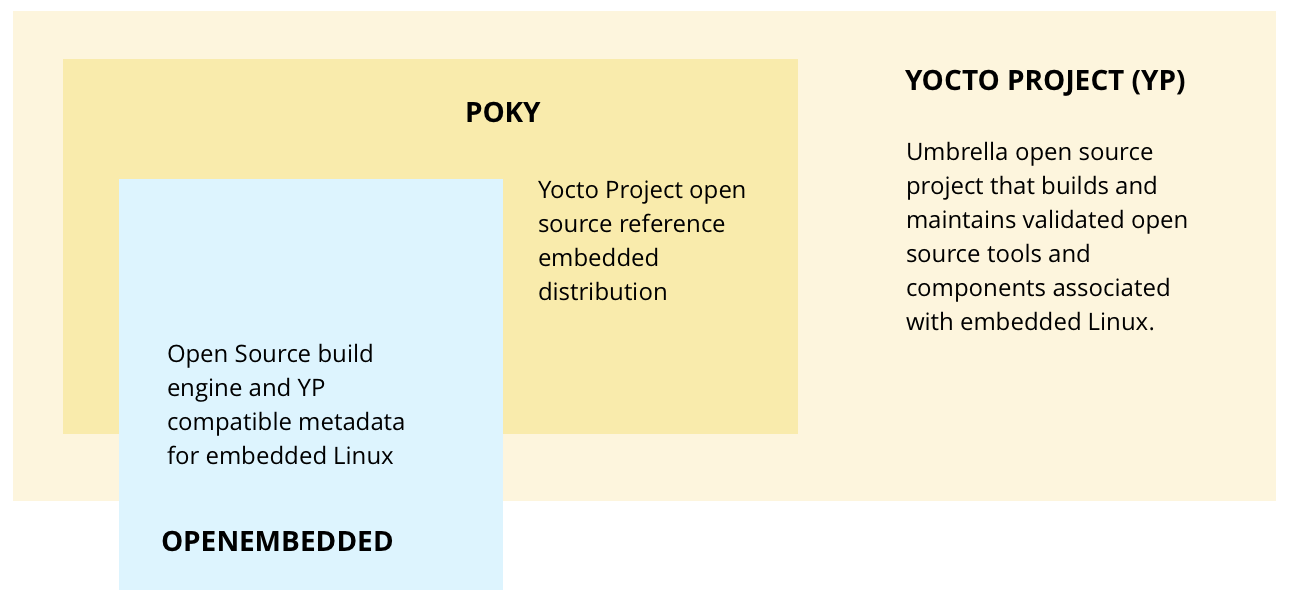
\includegraphics[width=0.60\linewidth]{figs/yocto-overview}
	\caption[Yocto Overview]{Esquema de relación entre Yocto, Poky y OpenEmbedded.}
	\label{fig:yocto_overview}
\end{figure}

\paragraph{}Al principio, Yocto puede resultar ser conceptualmente difícil de entender
ya que su campo de aplicación puede ser muy variado. En este sentido, puede usarse tanto
la creación de imágenes de completas de sistema, creación de \emph{\gls{bootloader}}, generación
de sistemas de ficheros (\emph{rootfs}), desarrollo de aplicativos, desarrollo de paquetes
de los aplicativos, desarrollo y/o hacking del kernel, generación de toolchain, \gls{SDK},
\gls{ADT}.

\paragraph{\label{layers} \label{recipes}}Los principales conceptos para enterder el funcionamiento de Yocto, son:
las capas o \emph{layers}, las recetas o \emph{recipes}, las clases y los ficheros de
configuración. Las \emph{recipes} son un conjunto de instrucciones y configuraciones
usados para la construcción de un paquete. Por ejemplo, una recipe describe la fuente
del código, los parámetros, el compilador, los parches a aplicar así como será la instalción
del paquete en la imagen. Las \emph{layers} son conjuntos de recipes agrupado por
funciones lógicas que funcionan de manera independiente o con una dependencia bien
documentada. Los ficheros de
%%%%%%%%%%%%%%%%%%%%%%%%%%%%%%%%%%%%%%%%%%%%%%




\paragraph{}En cuanto a las opciones de testing, Yocto está dispone de test en tiempo de compilación
así como la disposición de arrancar las imágenes generadas en una máquina virtual QEMU\ref{sec:qemu}.

\section{QEMU}\label{sec:qemu}

\paragraph{} Qemu es un emulador de hardware de código abierto capaz de interoperar con
\gls{KVM} para arrancar máquinas virtuales con un rendimiento casi nativo.
\cite{qemu}

\paragraph{}Qemu dispone de los siguientes modos de funcionamiento:

\begin{itemize}
	\item User-mode emulation
	\item System emulation
	\item \gls{KVM} Hosting
	\item Xen Hosting
\end{itemize}

\begin{figure}[h]
	\centering
	
\includegraphics[width=0.50\linewidth]{imgs/qemu-logo}
	\caption[Qemu Logo]{Logo de QEMU.}
	\label{fig:qemu}
\end{figure}

\paragraph{} El modo ``User-mode emulation'' permite que una sola aplicación compilada
para una arquitectura diferente a la del resto del sistema arranque mediante la "traducción"
de instrucciones en tiempo real.

\paragraph{} El modo ``System emulation'' es el más común. Se utiliza para simular una computadora
completa, incluidos sus periféricos. Qemu tiene la capacidad de albergar sistemas operativos
linux, Solaris, Microsoft Windows, DOS y BSD.

\paragraph{} Los modos ``\gls{KVM}'' y ``\gls{XEN}'' son variaciones del modo ``System emulation'' en el
que emulan más o menos hardware con cada uno de los hipervisores cuyo nombre coincide con
el nombre del modo.

\section{Docker}\label{sec:docker}

\paragraph{}Docker es una herramienta de gestión de contenedores. Dichos contenedores son
una capa de aislamiento a nivel de aplicación, utilizan los recursos del Kernel de Linux
tales como espacios de nombres. A pesar de que no supone un aislamiento tan fuerte como
el que proporcionan las máquinas virtuales, la principal ventaja de los contenedores es
que son mucho más livianos en cuanto necesidad de recursos de memoria, disco y computación.
\cite{docker}

\paragraph{} Docker permite empaquetar aplicaciones y todas sus dependencias, de esta
forma tienen una gran capacidad de protabilidad y flexibilidad con respecto al sistema
operativo dónde se ejecuten.

\begin{figure}[H]
	\centering
	
\includegraphics[width=0.50\linewidth]{imgs/docker-logo}
	\caption[Docker Logo]{Logo de Docker.}
	\label{fig:docker}
\end{figure}

\paragraph{} En nuestro caso, Docker nos va a ayudar a empaquetar todo el entorno de
desarrollo y sus dependencias para que su puesta en marcha sea inmediata, también buscará
evitar la heterogeneidad entre los entornos de desarrollo de los diferentes desarrolladores.


\section{Flutter}\label{sec:flutter}

\paragraph{} Flutter es un entorno de desarrollo o \gls{SDK} de aplicaciones. El principal
objetivo de Flutter es facilitar la creación de interfaces de usuario que se adapten a
cualquier pantalla y a cualquier dispositivo. En ese sentido, permite que con un sólo
código fuente común se puedan generar aplicaciones para muchos entornos: Android, iOS,
Linux, Windows, Fucsia, etc.
\cite{flutter}

\paragraph{} Sigue la filosofía de programación basada en objetos, y como está pensado
fundamentalmente para entornos gráficos, todos los objetos en Flutter son \gls{Widgets}.

\begin{figure}[h]
	\centering
	
\includegraphics[width=0.50\linewidth]{imgs/flutter-logo}
	\caption[Flutter Logo]{Logo de Flutter.}
	\label{fig:flutter}
\end{figure}

\paragraph{} Gracias a su capacidad para hacer el \gls{cross-compile} sencillo, resulta
ser increiblemente práctico para su uso en aplicaciones embebidas. Permite el desarrollo
de forma aislada del hardware así como el testing de la aplicación. En el apartado
gráfico destaca la persistencia visual entre la interfaz en entornos de desarrollo y
entornos embebidos.

\paragraph{} Está escrito en el lenguaje de programación Dart\ref{sec:dart} y ha sido
desarrollado por Google.

\subsection{Dart}\label{sec:dart}

\paragraph{}Dart es un lenguaje de programación orientado a objetos de alto nivel.
Está optimizado para interfaces de usuario y para aumentar la productividad de desarrollo,
ya que permite el ``hot debuging'', una técnica que permite cambiar sólo los objetos cuyo
codigo ha sido actualizado, manteniendo el resto en mitad de una sesión de depuración.
\cite{dart}

\paragraph{}Permite compilarse en código máquina para tener un rendimiento similar al
de aplicaciones nativas. Pero también puede traducirse a JavaScript para su uso en
entornos web. Todo eso lo convierte en un lenguaje de programación multiparadigma que
permite el desarrollo tanto del \gls{front-end} como del \gls{back-end}.

\begin{figure}[H]
	\centering
	
\includegraphics[width=0.50\linewidth]{imgs/dart-logo}
	\caption[Dart Logo]{Logo de Dart.}
	\label{fig:dart}
\end{figure}

\section{Qt}\label{sec:Qt}

\section{Ansible}\label{sec:ansible}

\section{Javascript con ReactJS}\label{sec:reactjs}

\section{Vagrant}\label{sec:vagrant}

%\subsection{Raspberri Pi 3.}

%\begin{figure}[h]
%	\centering
%	\includegraphics[width=0.55\linewidth]{imgs/rpi3}
%	\caption[Raspberry Pi 3]{Raspberry Pi 3}
%	\label{fig:rpi3}
%\end{figure}

%\begin{itemize}
%	\item Procesador 4 ncleos de 1,2 GHz ARM Cortex-A53.
%	\item GPU: Dual Core VideoCore IV  Multimedia Co-procesador. Proporciona Open GL ES 2.0, OpenVG acelerado por hardware, y 1080p30 H.264 de alto perfil de decodificacin.
%	\item Ethernet socket Ethernet 10/100 BaseT.
%	\item Salida de vdeo: HDMI rev 1.3 y 1.4
%	\item Conector GPIO:
%	\begin{itemize}
%		\item 40-clavijas de 2,54 mm
%		\item Proporcionar 27 pines GPIO, as como 3,3 V, +5 V y GND lneas de suministro.
%	\end{itemize}
%	\item Zcalo tarjetas SD. Con soporte para Linux.
%\end{itemize}

%\begin{figure}[h]
%	\centering
%	\includegraphics[width=0.6\linewidth]{imgs/datapathVSN900}
%	\caption[VSN900 de Datapath]{Modelo VSN900 de Datapath}
%	\label{fig:datapathvsn900}
%\end{figure}

%\begin{table}[hbt]
%	\label{t:Desglose}
%	\centering
%	\begin{tabular}{|c|c|c|c|}
%		\hline
%		\textbf{Elemento} & \textbf{Precio Und.[\euro]} & \textbf{N Unds} & \textbf{Total elemento [\euro]} \\
%		\hline
%		\textbf{Total} &  &  & 350 (50/display) \\
%		\hline
%	\end{tabular}
%	\caption{Desglose econmico de la caja.}
%\end{table}
